\subsection{Temperature}

\subsubsection{Descripción}

\begin{wrapfigure}{r}{0.3\textwidth}
	\centering
	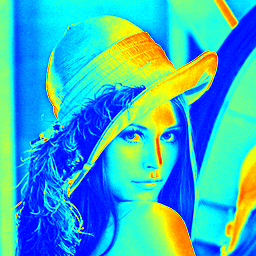
\includegraphics[width=0.3\textwidth]{imagenes/lenaTEMP.jpg}
\end{wrapfigure}

El filtro temperatura toma una imagen fuente y genera un efecto que simula un mapa de calor. Dicho efecto lo consigue tomando los tres componentes de color de cada pixel y promediándolos. Luego le asigna un valor que depende de este promedio \textit{t}.

\begin{center}
$\mathsf{t}_{(i,j)} = \lfloor(\mathsf{src}.r_{(i,j)} + \mathsf{src}.g_{(i,j)} + \mathsf{src}.b_{(i,j)}) / 3\rfloor$
\end{center}

Finalmente el color en la imagen destino se determina en función de la temperatura \textit{t} conforme al siguiente mapeo:

\begin{center}
\begin{displaymath}
\mathsf{dst}_{(i,j)}<r,g,b> = \left\{
\begin{array}{l l}
			<0,0, 128 + t \cdot 4> & \text{si }t < 32\\
			<0, (t - 32) \cdot 4, 255> & \text{si }32 \le t < 96\\
			<(t-96) \cdot 4, 255, 255 - (t-96) \cdot 4> & \text{si }96 \le t < 160\\
			<255, 255 - (t - 160) \cdot 4, 0> & \text{si }160 \le t < 224\\
			<255 - (t - 224) \cdot 4, 0 , 0> & \text{si no} \\
\end{array}
\right.
\end{displaymath}
\end{center}

\hfill
\subsubsection{Implementación C}

El algoritmo implementado en lenguaje C recorre la imagen iterativamente. Por cada pixel en la imagen original calcula el promedio de sus componentes RGB (línea 4) y según este valor se guarda en la imagen destino el calculo correspondiente a la temperatura (líneas 5 a 15). A continuación el pseudocódigo:
	
\begin{algorithm}[H]
  \begin{algorithmic}[1]
		\FORALL{y:=0 \TO  Height($I_{src}$)}
			\FORALL{x:=0 \TO  Width($I_{src}$)}
				\STATE $ pixel \gets I_{src}(x,y)$
				\STATE $Nat $ $ t \gets \lfloor(\frac{Red(pixel)+Green(pixel)+Blue(pixel)}{3}\rfloor$
				\IF{$t < 32$}
					\STATE $I_{dst}(x,y) \gets DevolverPixel(0,0,128+t \cdot 4)$
				\ELSIF{$ 32 \leq t < 96$}
					\STATE $I_{dst}(x,y) \gets DevolverPixel(0,(t-32) \cdot 4,255)$
				\ELSIF{$ 96 \leq t < 160$}
					\STATE $I_{dst}(x,y) \gets DevolverPixel((t-96) \cdot 4,255, 255-(t-96) \cdot 4)$
				\ELSIF{$ 160 \leq t < 224$}
					\STATE $I_{dst}(x,y) \gets DevolverPixel(255, 255-(t-160) \cdot 4, 0)$
				\ELSE		
					\STATE $I_{dst}(x,y) \gets DevolverPixel(255-(t-224) \cdot 4, 0, 0)$
				\ENDIF	
			\ENDFOR
		 \ENDFOR
  \end{algorithmic}
  \caption{$temperature (I_{src}, I_{dst})$}
  \label{alg:temperature}
\end{algorithm}	

\subsubsection{Implementación ASM}
En este filtro procesaremos de a 4 píxeles. Daremos la explicación de la partes más significativas del código assembler.

\subsubsection*{Cálculo del valor T}

En este tramo de código traigo los 4 píxeles de memoria. Desempaquetamps de Byte a Word en los registros XMM2 (parte baja) y XMM1 (parte alta). Después shifteamos 16 bits a izquierda y luego a derecha cada paquete de QWords para de esta manera tener el valor de la trasparencia en 0.

\begin{codesnippet}
\begin{verbatim}
    movdqu xmm0, [rdi]      ;Píxeles originales
    movdqu xmm1, xmm0       
    movdqu xmm2, xmm0

    pxor xmm7, xmm7         ; Masacara de ceros en xmm7 para desempaquetar de byte a word
    punpcklbw xmm2, xmm7    ; xmm2 = |a1 b1 g1 r1|a0 b0 g0 r0| parte baja
    punpckhbw xmm1, xmm7    ; xmm1 = |a3 b3 g3 r3|a2 b2 g2 r2| parte alta
                            ; Shifteo a izquierda para olvidarme del alfa
    psllq xmm1, 16          ; xmm1=|b3 g3 r3 0|b2 g2 r2 0|
    psllq xmm2, 16          ; xmm2=|b1 g1 r1 0|b0 g0 r0 0|
    psrlq xmm1, 16          ; xmm1=|0 b3 g3 r3|0 b2 g2 r2|
    psrlq xmm2, 16          ; xmm2=|0 b1 g1 r1|0 b0 g0 r0|
\end{verbatim}
\end{codesnippet}

Para calcular las sumas de la 3 componentes \emph{b+g+r}. Realizamos sumas horizontales con la intrucción \emph{phaddw} y colocamos las sumas en los registros XMM1 y XMM2.

\begin{codesnippet}
\begin{verbatim}
                       ; Sumas horizontal
    phaddw xmm2, xmm2  ; xmm2=|0+b1 g1+r1 0+b0 g0+r0|0+b1 g1+r1 0+b0 g0+r0|
    phaddw xmm1, xmm1  ; xmm1=|0+b3 g3+r3 0+b2 g2+r2| 0+b3 g3+r3 0+b2 g2+r2|

    phaddw xmm2, xmm2  ; xmm2 =|b1+g1+r1 b0+g0+r0 b1+g1+r1 b0+g0+r0|b1+g1+r1 b0+g0+r0 b1+g1+r1...
    phaddw xmm1, xmm1  ; xmm1 =|b3+g3+r3 b2+g2+r2 b3+g3+r3 b2+g2+r2|b3+g3+r3 b2+g2+r2 b3+g3+r3...
                       ; xmm2 =|s1 s0 s1 s0|s1 s0 s1 s0|
                       ; xmm1 =|s3 s2 s3 s2|s3 s2 s3 s2|
\end{verbatim}
\end{codesnippet}

El objetivo de este paso es obtener \emph{xmm1=$|s3|s2|s1|s0|$}, donde \emph{s3,s2,s1 y s0} son las sumas \emph{b+g+r} del píxel 3,..,píxel 1 respectivamente.

\begin{codesnippet}
\begin{verbatim}
    ;shuffle parte baja (bits 63 a 0) de los words, para reordenar las sumas s0,s1,s2ys3
                                  ; imm8 = 1 1 0 0
    pshufhw xmm2, xmm2, 01010000b ; xmm2=|s1 s0 s1 s0|s1 s1 s0 s0| 
    pshufhw xmm1, xmm1, 01010000b ; xmm1=|s3 s2 s3 s2|s3 s3 s2 s2|
                                  ;shuffle parte alta(bits 127 a 64) de los word
    pshuflw xmm2, xmm2, 01010000b ; xmm2=|s1 s1 s0 s0|s1 s1 s0 s0|
    pshuflw xmm1, xmm1, 01010000b ; xmm1=|s3 s3 s2 s2|s3 s3 s2 s2|
                                  ;shifteo a derecha c/paquete dobleWord 16 bits
    psrld xmm2, 16;               ; xmm2=|0 s1|0 s0|0 s1|0 s0| 
    psrld xmm1, 16                ; xmm1=|0 s3|0 s2|0 s3|0 s2| 
								  ; Que es lo mismo q decir
                                  ; xmm2=|s1|s0|s1|s0|
                                  ; xmm1=|s3|s2|s3|s2|
\end{verbatim}
\end{codesnippet}

El objetivo de este paso es obtener \emph{xmm1=$|s3|s2|s1|s0|$}. Para eso primero convertimos los paquetes de enteros de Doble Word a Floats usando la intrucción \emph{cvtdq2ps}. Luego usamos la funcion \emph{blendps}, que sive para mezclar los registos XMM1 y XMM2 según el valor que pongamos en la fuente número 2 (en este caso 0011b).

\begin{codesnippet}
\begin{verbatim}
                                ; Convierto los valores de xmm1 a float
    cvtdq2ps xmm1, xmm1         ; xmm1=|s3|s2|s3|s2|
    cvtdq2ps xmm2, xmm2         ; xmm2=|s1|s0|s1|s0|
                                ; mesclamos los registros xmm1 y xmm2 usando el blendps
    blendps xmm1, xmm2, 0011b   ; xmm1 =|s3|s2|s1|s0|
\end{verbatim}
\end{codesnippet}

En este último paso queremos obtener \emph{xmm1=$|t4|t3|t2|t1|$}. Para eso dividimos (cvtps2dq) cada paquete de floats por 3. Convertimos los Floats a enteros dobleWords (cvtps2dq). Después desempaquetamos de Doble Word a Words (packusdw) y de Word a Byte (packuswb). Como último paso usamos shuffle (pshufb), para permutar los paquetes de Bytes teniendo como máscara xmm10. 

\begin{codesnippet}
\begin{verbatim}
    ; <t, t, t, t>          t < 32   <0, 0, 0, 4t + 128>
                            ; Divido todo por 3
    divps xmm1, xmm8        ; xmm1 =|s3/3.0|s2/3.0|s1/3.0|s0/3.0| 
                            ; convierto de Float a dobleWord entero
    cvtps2dq xmm1, xmm1     ; xmm1 =|t3|t2|t1|t0|
                            ; desempaqueto de dobleWord a Word sin signo y con saturación
    packusdw xmm1, xmm1     ; xmm1 =|t3|t2|t1|t0|t3|t2|t1|t0|
                            ; desempaqueto Word sin signo y byte con saturación
    packuswb xmm1, xmm1     ; xmm1 =|t3|t2|t1|t0|t3|t2|t1|t0|t3|t2|t1|t0|t3|t2|t1|t0| 
                            ; xmm10=|3|3|3|3|2|2|2|2|1|1|1|1|0|0|0|0|
    pshufb xmm1, xmm10      ; xmm1 = |t3t3|t3|t3|t2|t2|t2|t2|t1|t1|t1|t1|t0|t0|t0|t0|
                            ; xmm1 = |t3 t3 t3 t3|t2 t2 t2 t2|t1 t1 t1 t1|t0 t0 t0 t0|
\end{verbatim}
\end{codesnippet}

\subsubsection*{Caso $t<32$}
El objetivo de este caso es obtner en \emph{xmm4=$|$0 0 0 4.t3+128$|$0 0 0 4.t2+128$|$0 0 0 4.t1+128$|$0 0 0 4.t0+128$|$}. Primero multiplicamos por 4. Luego sumamos 128 de manera tal me quede $4.t+128$. Shifteamos cada paquete de DobleWord a derecha 24 bits. Finalmente guardamos todo en el registro xmm4 (ver fragmento de código).

\begin{codesnippet}
\begin{verbatim}
                        ; Caso: t < 32    <0, 0, 0, 4t + 128>
    movdqu xmm4, xmm1   ; xmm4=|t3 t3 t3 t3|t2 t2 t2 t2|t1 t1 t1 t1|t0 t0 t0 t0|

    paddb  xmm4, xmm1   ; multiplico por 2
    paddb  xmm4, xmm1   ; multiplico por 3 y 4
    paddb  xmm4, xmm1
                        ; sumo 128 a cada byte de xmm4
                        ; xmm11=|128|128|128|128|128|128|128|128|128|128|128|128|128|128|128|128|
    paddb  xmm4, xmm11 

                        ; shifteo a derecha 24 bits a cada paquete de DobleWord
    psrld  xmm4, 24     ; xmm4=|0 0 0 4.t3+128|0 0 0 4.t2+128|0 0 0 4.t1+128|0 0 0 4.t0+128|
\end{verbatim}
\end{codesnippet}

\subsubsection*{Casos restantes}
Caso: $32 \leq t < 96$ \\
En este caso debemos obtener \emph{xmm5=$|$0 0 4.(t3-32) 255$|$...$|$0 0 4.(t0-32) 255$|$ }. 
La parte interezante es que usamos la instrucción \emph{pinserb}, que inserta el valor contenido en \emph{r9}.
\begin{codesnippet}
\begin{verbatim}				
                        ;xmm11=|128|128|128|128|128|128|128|128|128|128|128|128|128|128|128|128|
                        ;xmm4=|t3 t3 t3 t3|t2 t2 t2 t2|t1 t1 t1 t1|t0 t0 t0 t0|
    psubb xmm5, xmm11   ;xmm5=|4.t3-128 4.t3-128 4.t3-128 4.t3-128|...

    pinsrb xmm5, r9b, 12 ; xmm5=|4.(t3-32) 4.(t3-32) 4.(t3-32) 4.(t3-32)+255|...
    pinsrb xmm5, r9b, 8  
    pinsrb xmm5, r9b, 4
    pinsrb xmm5, r9b, 0  ;xmm5=|4.(t3-32) 4.(t3-32) 4.(t3-32) 255|...

    pslld xmm5, 16      ;xmm5=|4.(t3-32) 255 0 0|...|4.(t0-32) 255 0 0|
    psrld xmm5, 16      ;xmm5=|0 0 4.(t3-32) 255|...|0 0 4.(t0-32) 255|                    
\end{verbatim}
\end{codesnippet}

Casos restantes se resuelven de igual manera($96\leq t < 160$, $160\leq t <225$ y  $224 \leq t$).

\subsubsection*{Paso final}

Este es el último paso. Acá debemos quedarnos con las valores según valfa \emph{T}, Son todas operaciones lógicas y comparaciones. Solo debemos recordar q en xmm4,  xmm5, xmm6, xmm7 y xmm3 estan los casos T.

\begin{codesnippet}
\begin{verbatim}				
    psrld xmm1,  24    ; xmm1=|0 0 0 t3|0 0 0 0 t2|0 0 0 t1|0 0 0 t0|

    ; En este paso produzco todas las máscaras segun el valor de T

    pcmpgtd xmm12, xmm1     ; [32 > t?...] Me quedo con t < 32
    pcmpgtd xmm13, xmm1     ; [96 > t?...] Me quedo con t < 96
    pxor    xmm13, xmm12    ; Me quedo con 32 <= t < 96
    pcmpgtd xmm14, xmm1     ; [160 > t?...] Me quedo con t < 160
    pxor    xmm14, xmm12
    pxor    xmm14, xmm13    ; Me quedo con 96 <= t < 160
    pcmpgtd xmm15, xmm1     ; [224 > t?...] Me quedo con t < 224
    pxor    xmm15, xmm12
    pxor    xmm15, xmm13
    pxor    xmm15, xmm14    ; Me quedo con 160 <= t < 224    ; t > 224?
    pxor    xmm9,  xmm12
    pxor    xmm9,  xmm13
    pxor    xmm9,  xmm14
    pxor    xmm9,  xmm15

    ; utilizando las mascaras producidas en el paso anterior unimos todos los casos
    
    pand xmm12, xmm4        ; [t<32, 0, 0 , t<32, ...]
    pand xmm13, xmm5        ; [t<96, t <96, 0,...]
    pand xmm14, xmm3        ; [t<160, t<160, 0, 0 ,t<160]
    pand xmm15, xmm6        ; [t<224, t<224, 0, 0 ,t<224]
    pand  xmm9, xmm7        ; [t>224, t>224, 0, 0 ,t>224]
													
    por xmm12, xmm13
    por xmm12, xmm14
    por xmm12, xmm15
    por xmm12, xmm9        ;En xmm12 guardamos las 4 temperaturas del pixel.
\end{verbatim}
\end{codesnippet}

Resta copiar los valores de los 4 píxeles de \emph{xmm12} a memoria.